%%=============================================================================
%% LaTeX sjabloon voor bachelorproef, HoGent Bedrijf en Organisatie
%% Opleiding Toegepaste Informatica
%%=============================================================================

\documentclass[fleqn,a4paper,12pt]{book}

%%=============================================================================
%% LaTeX sjabloon voor de bachelorproef, HoGent Bedrijf en Organisatie
%% Opleiding toegepaste informatica
%%
%% Structuur en algemene vormgeving. Meestal hoef je hier niets te wijzigen.
%%
%% Vormgeving gebaseerd op "The Legrand Orange Book", version 2.0 (9/2/15)
%% door Mathias Legrand (legrand.mathias@gmail.com) met aanpassingen door
%% Vel (vel@latextemplates.com). Het oorspronkelijke template is te vinden op
%% http://www.LaTeXTemplates.com
%%
%% Aanpassingen voor HoGent toegepaste informatica: 
%%   Bert Van Vreckem <bert.vanvreckem@hogent.be>
%% Licentie: 
%%   CC BY-NC-SA 3.0 (http://creativecommons.org/licenses/by-nc-sa/3.0/)
%%=============================================================================

%%-----------------------------------------------------------------------------
%% Packages
%%-----------------------------------------------------------------------------

\usepackage[top=3cm,bottom=3cm,left=3cm,right=3cm,headsep=10pt,a4paper]{geometry} % Page margins
\usepackage[utf8]{inputenc}  % Accenten gebruiken in tekst (vb. é ipv \'e)
\usepackage{amsfonts}        % AMS math packages: extra wiskundige
\usepackage{amsmath}         %   symbolen (o.a. getallen-
\usepackage{amssymb}         %   verzamelingen N, R, Z, Q, etc.)
\usepackage[english,dutch]{babel}    % Taalinstellingen: woordsplitsingen,
                             %  commando's voor speciale karakters
                             %  ("dutch" voor NL)
\usepackage{iflang}
\usepackage{eurosym}         % Euro-symbool €
\usepackage{geometry}
\usepackage{graphicx}        % Invoegen van tekeningen
\graphicspath{{img/}}       % Specifies the directory where pictures are stored
\usepackage{tikz}            % Required for drawing custom shapes
\usepackage[pdftex,bookmarks=true]{hyperref}
                             % PDF krijgt klikbare links & verwijzingen,
                             %  inhoudstafel
\usepackage{enumitem}        % Customize lists
\setlist{nolistsep}         % Reduce spacing between list items
\usepackage{listings}        % Broncode mooi opmaken
\usepackage{multirow}        % Tekst over verschillende cellen in tabellen
\usepackage{rotating}        % Tabellen en figuren roteren

\usepackage{booktabs}        % Required for nicer horizontal rules in tables

\usepackage[normalem]{ulem}
\useunder{\uline}{\ul}{}
\usepackage{lscape}
\usepackage{longtable}

\usepackage{xcolor}          % Required for specifying colors by name
\definecolor{maincolor}{RGB}{0,147,208} % Define the main color used for 
                             % highlighting throughout the book
                             % 0, 147, 208 = officiële kleur HoGent FBO

% Paragraph style: no indent, add space between paragraphs
\setlength{\parindent}{0em}
\setlength{\parskip}{1em}

\usepackage{etoolbox}
\usepackage{titling} % Macros for title, author, etc
\usepackage{lipsum}          % Voor vultekst (lorem ipsum)

%----------------------------------------------------------------------------------------
%	FONTS
%----------------------------------------------------------------------------------------

\usepackage{avant} % Use the Avantgarde font for headings
%\usepackage{times} % Use the Times font for headings
\usepackage{mathptmx} % Use the Adobe Times Roman as the default text font together with math symbols from the Sym­bol, Chancery and Com­puter Modern fonts

\usepackage{microtype} % Slightly tweak font spacing for aesthetics
\usepackage[utf8]{inputenc} % Required for including letters with accents
\usepackage[T1]{fontenc} % Use 8-bit encoding that has 256 glyphs

%------------------------------------------------------------------------------
%	TITLE PAGE
%------------------------------------------------------------------------------

\newcommand{\inserttitlepage}{%
\begin{titlepage}
  \newgeometry{top=2cm,bottom=1.5cm,left=1.5cm,right=1.5cm}
  \begin{center}

    \begingroup
    \rmfamily
    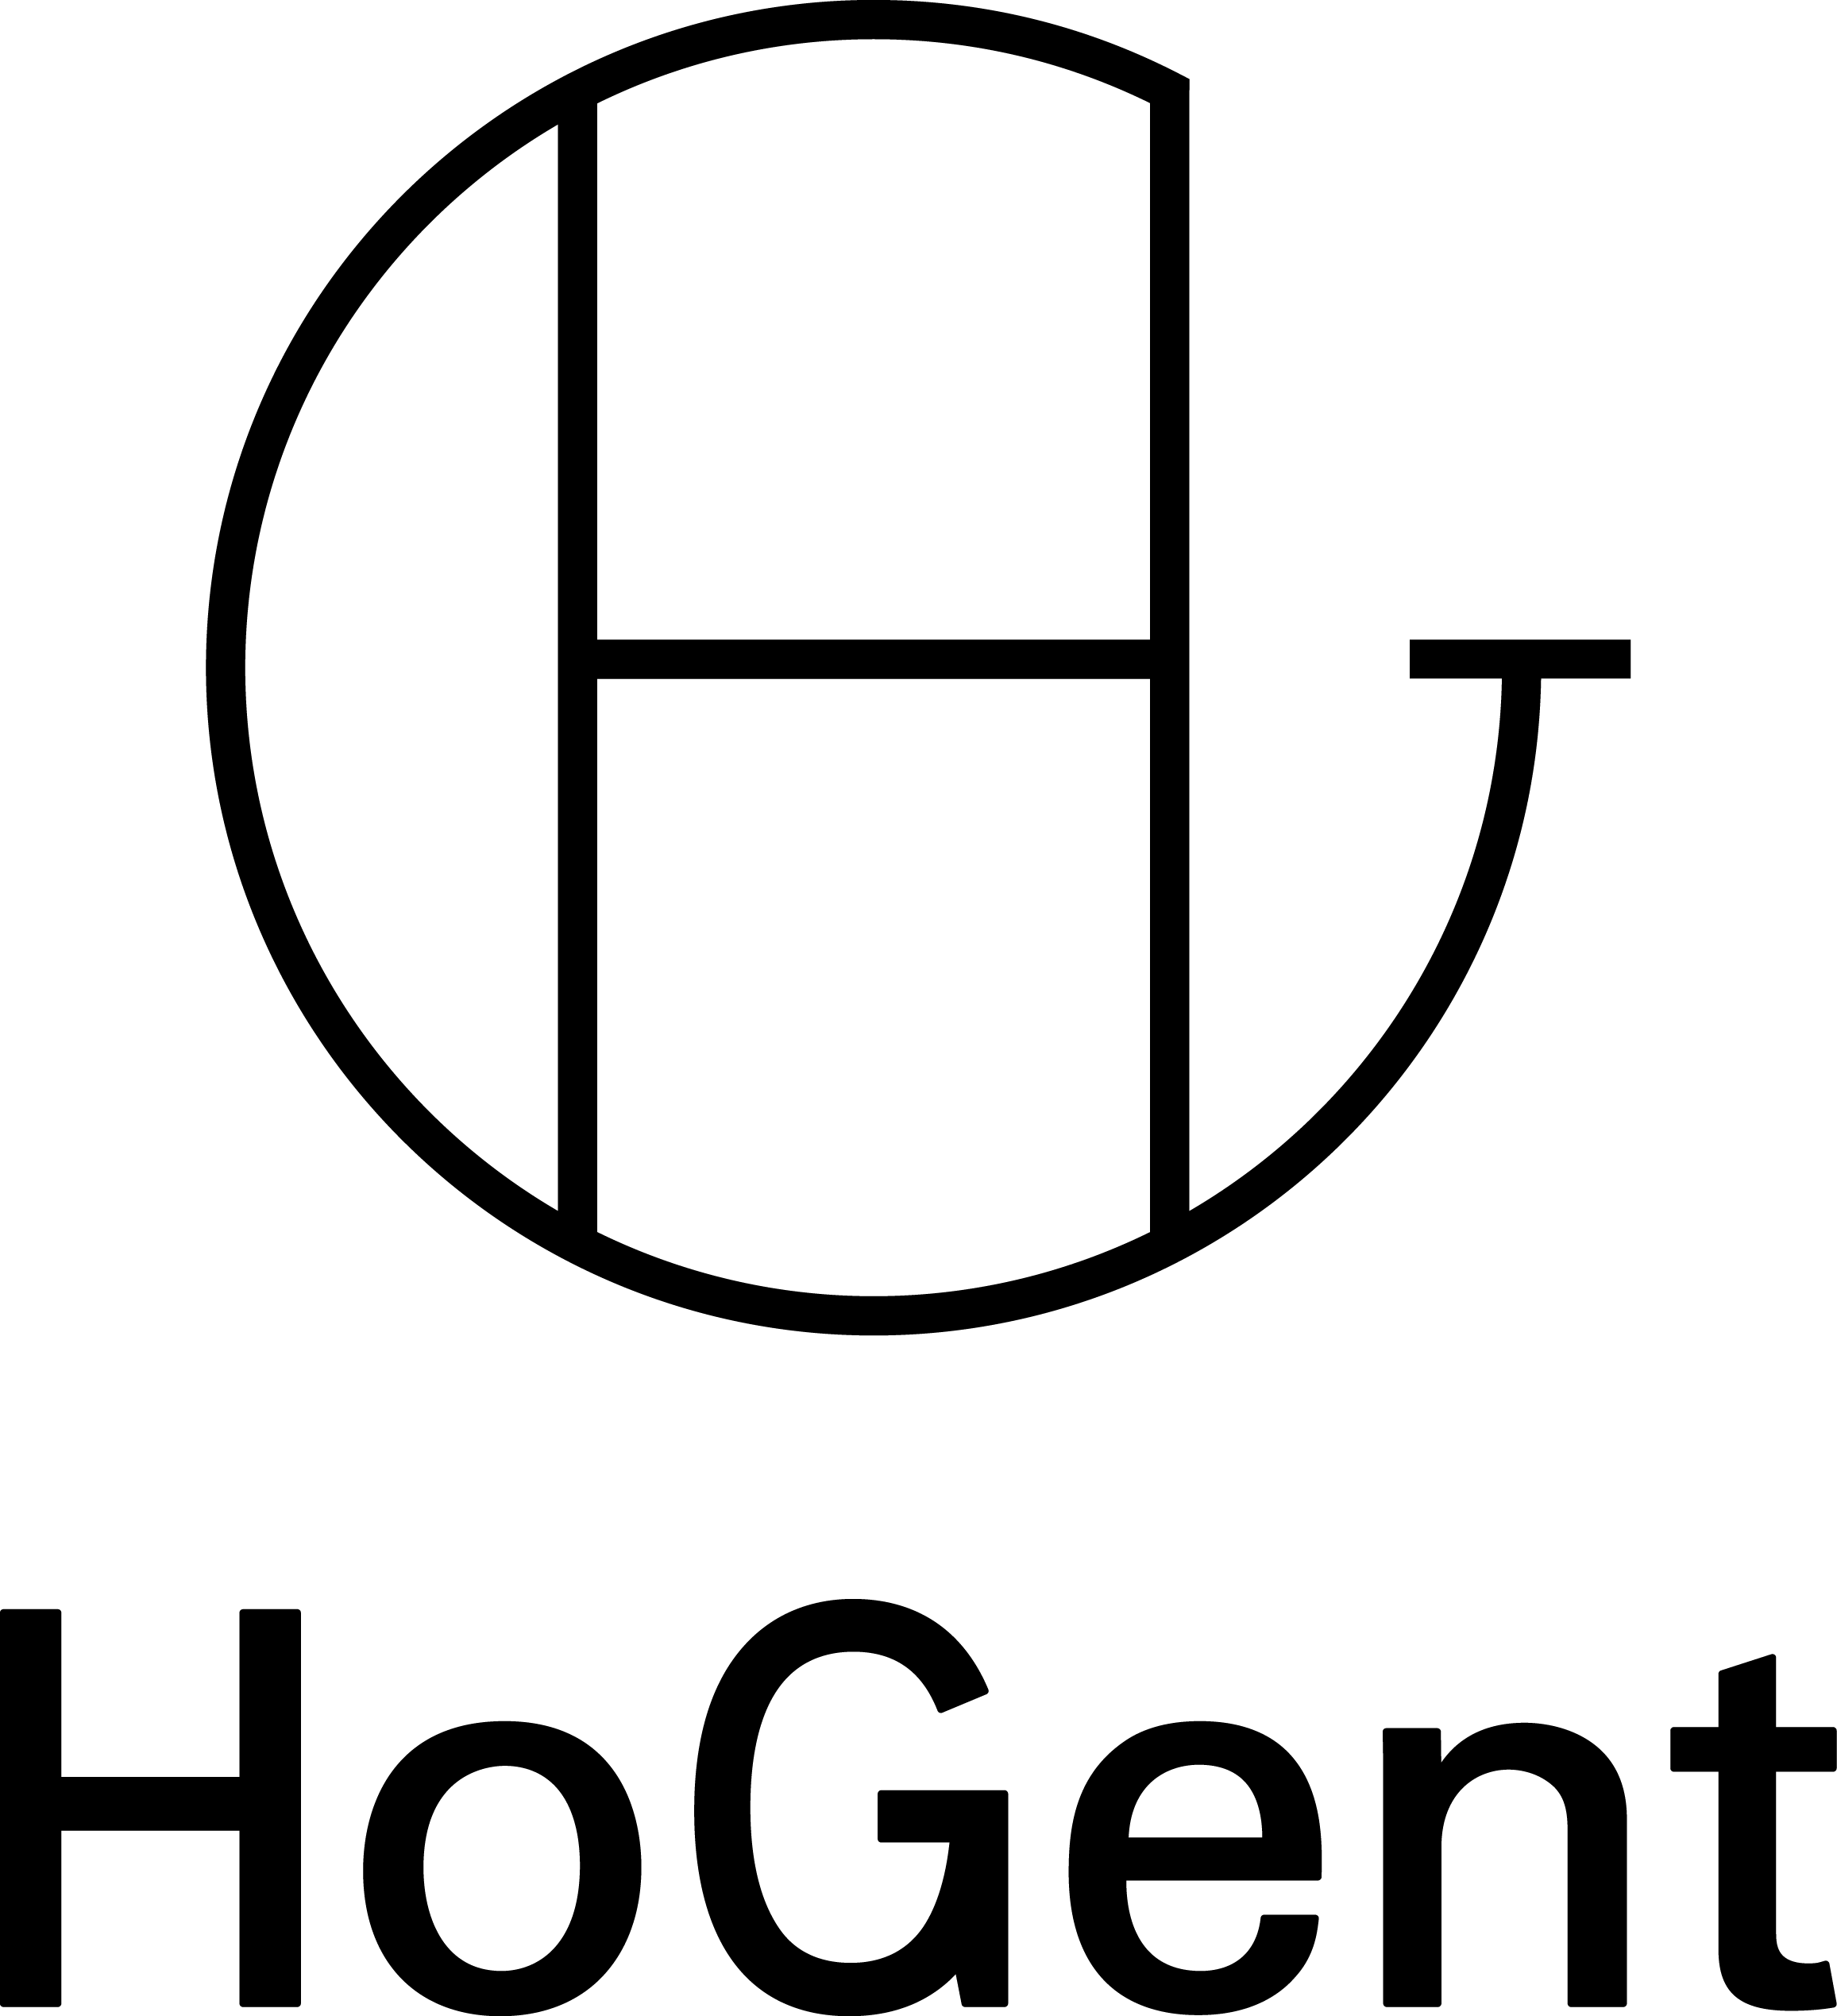
\includegraphics[width=2.5cm]{img/HG-beeldmerk-woordmerk}\\[.5cm]
    Faculteit Bedrijf en Organisatie\\[3cm]
    \titel
    \vfill
    \student\\[3.5cm]
    Scriptie voorgedragen tot het bekomen van de graad van\\professionele bachelor in de toegepaste informatica\\[2cm]
    Promotor:\\
    \promotor\\
    \ifdefempty{\copromotor}{\vspace{2.5cm}}{Co-promotor:\\\copromotor\\[2.5cm]}
    Instelling: \instelling\\[.5cm]
    Academiejaar: \academiejaar\\[.5cm]
    \ifcase \examenperiode \or Eerste \or Tweede \else Derde \fi examenperiode
    \endgroup

  \end{center}
  \restoregeometry
\end{titlepage}
  \emptypage
\begin{titlepage}
  \newgeometry{top=5.35cm,bottom=1.5cm,left=1.5cm,right=1.5cm}
  \begin{center}

    \begingroup
    \rmfamily
    \IfLanguageName{dutch}{Faculteit Bedrijf en Organisatie}{Faculty of Business and Information Management}\\[3cm]
    \titel
    \vfill
    \student\\[3.5cm]
    \IfLanguageName{dutch}{Scriptie voorgedragen tot het bekomen van de graad van\\professionele bachelor in de toegepaste informatica}{Thesis submitted in partial fulfilment of the requirements for the degree of\\professional bachelor of applied computer science}\\[2cm]
    Promotor:\\
    \promotor\\
    \ifdefempty{\copromotor}{\vspace{2.5cm}}{Co-promotor:\\\copromotor\\[2.5cm]}
    \IfLanguageName{dutch}{Instelling}{Institution}: \instelling\\[.5cm]
    \IfLanguageName{dutch}{Academiejaar}{Academic year}: \academiejaar\\[.5cm]
    \IfLanguageName{dutch}{%
    \ifcase \examenperiode \or Eerste \or Tweede \else Derde \fi examenperiode}{%
    \ifcase \examenperiode \or First \or Second \else Third \fi examination period}
    \endgroup

  \end{center}
  \restoregeometry
\end{titlepage}
}

%----------------------------------------------------------------------------------------
%	BIBLIOGRAPHY AND INDEX
%----------------------------------------------------------------------------------------

\usepackage[style=apa,backend=biber]{biblatex}
\usepackage{csquotes}
\DeclareLanguageMapping{dutch}{dutch-apa}
\addbibresource{bachproef-tin.bib} % BibTeX bibliography file
\addbibresource{../voorstel/voorstel.bib}
\defbibheading{bibempty}{}

\usepackage{calc} % For simpler calculation - used for spacing the index letter headings correctly
\usepackage{makeidx} % Required to make an index
\makeindex % Tells LaTeX to create the files required for indexing

%----------------------------------------------------------------------------------------
%	MAIN TABLE OF CONTENTS
%----------------------------------------------------------------------------------------

\usepackage{titletoc} % Required for manipulating the table of contents

\contentsmargin{0cm} % Removes the default margin

% Part text styling
\titlecontents{part}[0cm]
{\addvspace{20pt}\centering\large\bfseries}
{}
{}
{}

% Chapter text styling
\titlecontents{chapter}[1.25cm] % Indentation
{\addvspace{12pt}\large\sffamily\bfseries} % Spacing and font options for chapters
{\color{maincolor!60}\contentslabel[\Large\thecontentslabel]{1.25cm}\color{maincolor}} % Chapter number
{\color{maincolor}}
{\color{maincolor!60}\normalsize\;\titlerule*[.5pc]{.}\;\thecontentspage} % Page number

% Section text styling
\titlecontents{section}[1.25cm] % Indentation
{\addvspace{3pt}\sffamily\bfseries} % Spacing and font options for sections
{\contentslabel[\thecontentslabel]{1.25cm}} % Section number
{}
{\hfill\color{black}\thecontentspage} % Page number
[]

% Subsection text styling
\titlecontents{subsection}[1.25cm] % Indentation
{\addvspace{1pt}\sffamily\small} % Spacing and font options for subsections
{\contentslabel[\thecontentslabel]{1.25cm}} % Subsection number
{}
{\ \titlerule*[.5pc]{.}\;\thecontentspage} % Page number
[]

% List of figures
\titlecontents{figure}[0em]
{\addvspace{-5pt}\sffamily}
{\thecontentslabel\hspace*{1em}}
{}
{\ \titlerule*[.5pc]{.}\;\thecontentspage}
[]

% List of tables
\titlecontents{table}[0em]
{\addvspace{-5pt}\sffamily}
{\thecontentslabel\hspace*{1em}}
{}
{\ \titlerule*[.5pc]{.}\;\thecontentspage}
[]

%----------------------------------------------------------------------------------------
%	MINI TABLE OF CONTENTS IN PART HEADS
%----------------------------------------------------------------------------------------

% Chapter text styling
\titlecontents{lchapter}[0em] % Indenting
{\addvspace{15pt}\large\sffamily\bfseries} % Spacing and font options for chapters
{\color{maincolor}\contentslabel[\Large\thecontentslabel]{1.25cm}\color{maincolor}} % Chapter number
{}
{\color{maincolor}\normalsize\sffamily\bfseries\;\titlerule*[.5pc]{.}\;\thecontentspage} % Page number

% Section text styling
\titlecontents{lsection}[0em] % Indenting
{\sffamily\small} % Spacing and font options for sections
{\contentslabel[\thecontentslabel]{1.25cm}} % Section number
{}
{}

% Subsection text styling
\titlecontents{lsubsection}[.5em] % Indentation
{\normalfont\footnotesize\sffamily} % Font settings
{}
{}
{}

%----------------------------------------------------------------------------------------
%	PAGE HEADERS
%----------------------------------------------------------------------------------------

\usepackage{fancyhdr} % Required for header and footer configuration

\pagestyle{fancy}
\renewcommand{\chaptermark}[1]{\markboth{\sffamily\normalsize\bfseries\chaptername\ \thechapter.\ #1}{}} % Chapter text font settings
\renewcommand{\sectionmark}[1]{\markright{\sffamily\normalsize\thesection\hspace{5pt}#1}{}} % Section text font settings
\fancyhf{} \fancyhead[LE,RO]{\sffamily\normalsize\thepage} % Font setting for the page number in the header
\fancyhead[LO]{\rightmark} % Print the nearest section name on the left side of odd pages
\fancyhead[RE]{\leftmark} % Print the current chapter name on the right side of even pages
\renewcommand{\headrulewidth}{0.5pt} % Width of the rule under the header
\addtolength{\headheight}{2.5pt} % Increase the spacing around the header slightly
\renewcommand{\footrulewidth}{0pt} % Removes the rule in the footer
\fancypagestyle{plain}{\fancyhead{}\renewcommand{\headrulewidth}{0pt}} % Style for when a plain pagestyle is specified

% Removes the header from odd empty pages at the end of chapters
\makeatletter
\renewcommand{\cleardoublepage}{
\clearpage\ifodd\c@page\else
\hbox{}
\vspace*{\fill}
\thispagestyle{empty}
\newpage
\fi}

%----------------------------------------------------------------------------------------
%	THEOREM STYLES
%----------------------------------------------------------------------------------------

\usepackage{amsmath,amsfonts,amssymb,amsthm} % For math equations, theorems, symbols, etc

\newcommand{\intoo}[2]{\mathopen{]}#1\,;#2\mathclose{[}}
\newcommand{\ud}{\mathop{\mathrm{{}d}}\mathopen{}}
\newcommand{\intff}[2]{\mathopen{[}#1\,;#2\mathclose{]}}
\newtheorem{notation}{Notation}[chapter]

% Boxed/framed environments
\newtheoremstyle{maincolornumbox}% % Theorem style name
{0pt}% Space above
{0pt}% Space below
{\normalfont}% % Body font
{}% Indent amount
{\small\bf\sffamily\color{maincolor}}% % Theorem head font
{\;}% Punctuation after theorem head
{0.25em}% Space after theorem head
{\small\sffamily\color{maincolor}\thmname{#1}\nobreakspace\thmnumber{\@ifnotempty{#1}{}\@upn{#2}}% Theorem text (e.g. Theorem 2.1)
\thmnote{\nobreakspace\the\thm@notefont\sffamily\bfseries\color{black}---\nobreakspace#3.}} % Optional theorem note
\renewcommand{\qedsymbol}{$\blacksquare$}% Optional qed square

\newtheoremstyle{blacknumex}% Theorem style name
{5pt}% Space above
{5pt}% Space below
{\normalfont}% Body font
{} % Indent amount
{\small\bf\sffamily}% Theorem head font
{\;}% Punctuation after theorem head
{0.25em}% Space after theorem head
{\small\sffamily{\tiny\ensuremath{\blacksquare}}\nobreakspace\thmname{#1}\nobreakspace\thmnumber{\@ifnotempty{#1}{}\@upn{#2}}% Theorem text (e.g. Theorem 2.1)
\thmnote{\nobreakspace\the\thm@notefont\sffamily\bfseries---\nobreakspace#3.}}% Optional theorem note

\newtheoremstyle{blacknumbox} % Theorem style name
{0pt}% Space above
{0pt}% Space below
{\normalfont}% Body font
{}% Indent amount
{\small\bf\sffamily}% Theorem head font
{\;}% Punctuation after theorem head
{0.25em}% Space after theorem head
{\small\sffamily\thmname{#1}\nobreakspace\thmnumber{\@ifnotempty{#1}{}\@upn{#2}}% Theorem text (e.g. Theorem 2.1)
\thmnote{\nobreakspace\the\thm@notefont\sffamily\bfseries---\nobreakspace#3.}}% Optional theorem note

% Non-boxed/non-framed environments
\newtheoremstyle{maincolornum}% % Theorem style name
{5pt}% Space above
{5pt}% Space below
{\normalfont}% % Body font
{}% Indent amount
{\small\bf\sffamily\color{maincolor}}% % Theorem head font
{\;}% Punctuation after theorem head
{0.25em}% Space after theorem head
{\small\sffamily\color{maincolor}\thmname{#1}\nobreakspace\thmnumber{\@ifnotempty{#1}{}\@upn{#2}}% Theorem text (e.g. Theorem 2.1)
\thmnote{\nobreakspace\the\thm@notefont\sffamily\bfseries\color{black}---\nobreakspace#3.}} % Optional theorem note
\renewcommand{\qedsymbol}{$\blacksquare$}% Optional qed square
\makeatother

% Defines the theorem text style for each type of theorem to one of the three styles above
\newcounter{dummy}
\numberwithin{dummy}{section}
\theoremstyle{maincolornumbox}
\newtheorem{theoremeT}[dummy]{Theorem}
\newtheorem{problem}{Problem}[chapter]
\newtheorem{exerciseT}{Exercise}[chapter]
\theoremstyle{blacknumex}
\newtheorem{exampleT}{Example}[chapter]
\theoremstyle{blacknumbox}
\newtheorem{vocabulary}{Vocabulary}[chapter]
\newtheorem{definitionT}{Definition}[section]
\newtheorem{corollaryT}[dummy]{Corollary}
\theoremstyle{maincolornum}
\newtheorem{proposition}[dummy]{Proposition}

%----------------------------------------------------------------------------------------
%	DEFINITION OF COLORED BOXES
%----------------------------------------------------------------------------------------

\RequirePackage[framemethod=default]{mdframed} % Required for creating the theorem, definition, exercise and corollary boxes

% Theorem box
\newmdenv[skipabove=7pt,
skipbelow=7pt,
backgroundcolor=black!5,
linecolor=maincolor,
innerleftmargin=5pt,
innerrightmargin=5pt,
innertopmargin=5pt,
leftmargin=0cm,
rightmargin=0cm,
innerbottommargin=5pt]{tBox}

% Exercise box
\newmdenv[skipabove=7pt,
skipbelow=7pt,
rightline=false,
leftline=true,
topline=false,
bottomline=false,
backgroundcolor=maincolor!10,
linecolor=maincolor,
innerleftmargin=5pt,
innerrightmargin=5pt,
innertopmargin=5pt,
innerbottommargin=5pt,
leftmargin=0cm,
rightmargin=0cm,
linewidth=4pt]{eBox}

% Definition box
\newmdenv[skipabove=7pt,
skipbelow=7pt,
rightline=false,
leftline=true,
topline=false,
bottomline=false,
linecolor=maincolor,
innerleftmargin=5pt,
innerrightmargin=5pt,
innertopmargin=0pt,
leftmargin=0cm,
rightmargin=0cm,
linewidth=4pt,
innerbottommargin=0pt]{dBox}

% Corollary box
\newmdenv[skipabove=7pt,
skipbelow=7pt,
rightline=false,
leftline=true,
topline=false,
bottomline=false,
linecolor=gray,
backgroundcolor=black!5,
innerleftmargin=5pt,
innerrightmargin=5pt,
innertopmargin=5pt,
leftmargin=0cm,
rightmargin=0cm,
linewidth=4pt,
innerbottommargin=5pt]{cBox}

% Creates an environment for each type of theorem and assigns it a theorem text style from the "Theorem Styles" section above and a colored box from above
\newenvironment{theorem}{\begin{tBox}\begin{theoremeT}}{\end{theoremeT}\end{tBox}}
\newenvironment{exercise}{\begin{eBox}\begin{exerciseT}}{\hfill{\color{maincolor}\tiny\ensuremath{\blacksquare}}\end{exerciseT}\end{eBox}}
\newenvironment{definition}{\begin{dBox}\begin{definitionT}}{\end{definitionT}\end{dBox}}
\newenvironment{example}{\begin{exampleT}}{\hfill{\tiny\ensuremath{\blacksquare}}\end{exampleT}}
\newenvironment{corollary}{\begin{cBox}\begin{corollaryT}}{\end{corollaryT}\end{cBox}}

%----------------------------------------------------------------------------------------
%	REMARK ENVIRONMENT
%----------------------------------------------------------------------------------------

\newenvironment{remark}{\par\vspace{10pt}\small % Vertical white space above the remark and smaller font size
\begin{list}{}{
\leftmargin=35pt % Indentation on the left
\rightmargin=25pt}\item\ignorespaces % Indentation on the right
\makebox[-2.5pt]{\begin{tikzpicture}[overlay]
\node[draw=maincolor!60,line width=1pt,circle,fill=maincolor!25,font=\sffamily\bfseries,inner sep=2pt,outer sep=0pt] at (-15pt,0pt){\textcolor{maincolor}{R}};\end{tikzpicture}} % Orange R in a circle
\advance\baselineskip -1pt}{\end{list}\vskip5pt} % Tighter line spacing and white space after remark

%----------------------------------------------------------------------------------------
%	SECTION NUMBERING IN THE MARGIN
%----------------------------------------------------------------------------------------

\makeatletter
\renewcommand{\@seccntformat}[1]{\llap{\textcolor{maincolor}{\csname the#1\endcsname}\hspace{1em}}}
\renewcommand{\section}{\@startsection{section}{1}{\z@}
{-4ex \@plus -1ex \@minus -.4ex}
{1ex \@plus.2ex }
{\normalfont\large\sffamily\bfseries}}
\renewcommand{\subsection}{\@startsection {subsection}{2}{\z@}
{-3ex \@plus -0.1ex \@minus -.4ex}
{0.5ex \@plus.2ex }
{\normalfont\sffamily\bfseries}}
\renewcommand{\subsubsection}{\@startsection {subsubsection}{3}{\z@}
{-2ex \@plus -0.1ex \@minus -.2ex}
{.2ex \@plus.2ex }
{\normalfont\small\sffamily\bfseries}}
\renewcommand\paragraph{\@startsection{paragraph}{4}{\z@}
{-2ex \@plus-.2ex \@minus .2ex}
{.1ex}
{\normalfont\small\sffamily\bfseries}}

%----------------------------------------------------------------------------------------
%	PART HEADINGS
%----------------------------------------------------------------------------------------

% numbered part in the table of contents
\newcommand{\@mypartnumtocformat}[2]{%
\setlength\fboxsep{0pt}%
\noindent\colorbox{maincolor!20}{\strut\parbox[c][.7cm]{\ecart}{\color{maincolor!70}\Large\sffamily\bfseries\centering#1}}\hskip\esp\colorbox{maincolor!40}{\strut\parbox[c][.7cm]{\linewidth-\ecart-\esp}{\Large\sffamily\centering#2}}}%
%%%%%%%%%%%%%%%%%%%%%%%%%%%%%%%%%%
% unnumbered part in the table of contents
\newcommand{\@myparttocformat}[1]{%
\setlength\fboxsep{0pt}%
\noindent\colorbox{maincolor!40}{\strut\parbox[c][.7cm]{\linewidth}{\Large\sffamily\centering#1}}}%
%%%%%%%%%%%%%%%%%%%%%%%%%%%%%%%%%%
\newlength\esp
\setlength\esp{4pt}
\newlength\ecart
\setlength\ecart{1.2cm-\esp}
\newcommand{\thepartimage}{}%
\newcommand{\partimage}[1]{\renewcommand{\thepartimage}{#1}}%
\def\@part[#1]#2{%
\ifnum \c@secnumdepth >-2\relax%
\refstepcounter{part}%
\addcontentsline{toc}{part}{\texorpdfstring{\protect\@mypartnumtocformat{\thepart}{#1}}{\partname~\thepart\ ---\ #1}}
\else%
\addcontentsline{toc}{part}{\texorpdfstring{\protect\@myparttocformat{#1}}{#1}}%
\fi%
\startcontents%
\markboth{}{}%
{\thispagestyle{empty}%
\begin{tikzpicture}[remember picture,overlay]%
\node at (current page.north west){\begin{tikzpicture}[remember picture,overlay]%
\fill[maincolor!20](0cm,0cm) rectangle (\paperwidth,-\paperheight);
\node[anchor=north] at (4cm,-3.25cm){\color{maincolor!40}\fontsize{220}{100}\sffamily\bfseries\@Roman\c@part};
\node[anchor=south east] at (\paperwidth-1cm,-\paperheight+1cm){\parbox[t][][t]{8.5cm}{
\printcontents{l}{0}{\setcounter{tocdepth}{1}}%
}};
\node[anchor=north east] at (\paperwidth-1.5cm,-3.25cm){\parbox[t][][t]{15cm}{\strut\raggedleft\color{white}\fontsize{30}{30}\sffamily\bfseries#2}};
\end{tikzpicture}};
\end{tikzpicture}}%
\@endpart}
\def\@spart#1{%
\startcontents%
\phantomsection
{\thispagestyle{empty}%
\begin{tikzpicture}[remember picture,overlay]%
\node at (current page.north west){\begin{tikzpicture}[remember picture,overlay]%
\fill[maincolor!20](0cm,0cm) rectangle (\paperwidth,-\paperheight);
\node[anchor=north east] at (\paperwidth-1.5cm,-3.25cm){\parbox[t][][t]{15cm}{\strut\raggedleft\color{white}\fontsize{30}{30}\sffamily\bfseries#1}};
\end{tikzpicture}};
\end{tikzpicture}}
\addcontentsline{toc}{part}{\texorpdfstring{%
\setlength\fboxsep{0pt}%
\noindent\protect\colorbox{maincolor!40}{\strut\protect\parbox[c][.7cm]{\linewidth}{\Large\sffamily\protect\centering #1\quad\mbox{}}}}{#1}}%
\@endpart}
\def\@endpart{\vfil\newpage
\if@twoside
\if@openright
\null
\thispagestyle{empty}%
\newpage
\fi
\fi
\if@tempswa
\twocolumn
\fi}

%----------------------------------------------------------------------------------------
%	CHAPTER HEADINGS
%----------------------------------------------------------------------------------------

% A switch to conditionally include a picture, implemented by  Christian Hupfer
\newif\ifusechapterimage
\usechapterimagetrue
\newcommand{\thechapterimage}{}%
\newcommand{\chapterimage}[1]{\ifusechapterimage\renewcommand{\thechapterimage}{#1}\fi}%
\def\@makechapterhead#1{%
{\parindent \z@ \raggedright \normalfont
\ifnum \c@secnumdepth >\m@ne
\if@mainmatter
\begin{tikzpicture}[remember picture,overlay]
\node at (current page.north west)
{\begin{tikzpicture}[remember picture,overlay]
\node[anchor=north west,inner sep=0pt] at (0,0) {\ifusechapterimage\includegraphics[width=\paperwidth]{\thechapterimage}\fi};
\draw[anchor=west] (\Gm@lmargin,-9cm) node [line width=2pt,rounded corners=15pt,draw=maincolor,fill=white,fill opacity=0.5,inner sep=15pt]{\strut\makebox[22cm]{}};
\draw[anchor=west] (\Gm@lmargin+.3cm,-9cm) node {\huge\sffamily\bfseries\color{black}\thechapter. #1\strut};
\end{tikzpicture}};
\end{tikzpicture}
\else
\begin{tikzpicture}[remember picture,overlay]
\node at (current page.north west)
{\begin{tikzpicture}[remember picture,overlay]
\node[anchor=north west,inner sep=0pt] at (0,0) {\ifusechapterimage\includegraphics[width=\paperwidth]{\thechapterimage}\fi};
\draw[anchor=west] (\Gm@lmargin,-9cm) node [line width=2pt,rounded corners=15pt,draw=maincolor,fill=white,fill opacity=0.5,inner sep=15pt]{\strut\makebox[22cm]{}};
\draw[anchor=west] (\Gm@lmargin+.3cm,-9cm) node {\huge\sffamily\bfseries\color{black}#1\strut};
\end{tikzpicture}};
\end{tikzpicture}
\fi\fi\par\vspace*{270\p@}}}

%-------------------------------------------

\def\@makeschapterhead#1{%
\begin{tikzpicture}[remember picture,overlay]
\node at (current page.north west)
{\begin{tikzpicture}[remember picture,overlay]
\node[anchor=north west,inner sep=0pt] at (0,0) {\ifusechapterimage\includegraphics[width=\paperwidth]{\thechapterimage}\fi};
\draw[anchor=west] (\Gm@lmargin,-9cm) node [line width=2pt,rounded corners=15pt,draw=maincolor,fill=white,fill opacity=0.5,inner sep=15pt]{\strut\makebox[22cm]{}};
\draw[anchor=west] (\Gm@lmargin+.3cm,-9cm) node {\huge\sffamily\bfseries\color{black}#1\strut};
\end{tikzpicture}};
\end{tikzpicture}
\par\vspace*{270\p@}}
\makeatother

%----------------------------------------------------------------------------------------
%	HYPERLINKS IN THE DOCUMENTS
%----------------------------------------------------------------------------------------

\usepackage{hyperref}
\hypersetup{hidelinks,backref=true,pagebackref=true,hyperindex=true,colorlinks=false,breaklinks=true,urlcolor= maincolor,bookmarks=true,bookmarksopen=false,pdftitle={Title},pdfauthor={Author}}
\usepackage{bookmark}
\bookmarksetup{
open,
numbered,
addtohook={%
\ifnum\bookmarkget{level}=0 % chapter
\bookmarksetup{bold}%
\fi
\ifnum\bookmarkget{level}=-1 % part
\bookmarksetup{color=maincolor,bold}%
\fi
}
}

%----------------------------------------------------------------------------------------
%	Java source code
%----------------------------------------------------------------------------------------

% Commando voor invoegen Java-broncodebestanden (dank aan Niels Corneille)
% Gebruik:
%   \codefragment{source/MijnKlasse.java}{Uitleg bij de code}
%
% Je kan dit aanpassen aan de taal die je zelf het meeste gebruikt in je
% bachelorproef.
\newcommand{\codefragment}[2]{ \lstset{%
  language=java,
  breaklines=true,
  float=th,
  caption={#2},
  basicstyle=\scriptsize,
  frame=single,
  extendedchars=\true
}
\lstinputlisting{#1}}

% Leeg blad
\newcommand{\emptypage}{%
\newpage
\thispagestyle{empty}
\mbox{}
\newpage
}


%%---------- Documenteigenschappen --------------------------------------------
%% TODO: Vul dit aan met je eigen info:

% Je eigen naam
\newcommand{\student}{Piet Pieters}

% De naam van je promotor (lector van de opleiding)
\newcommand{\promotor}{Bert Van Vreckem}

% De naam van je co-promotor. Als je promotor ook je opdrachtgever is en je
% dus ook inhoudelijk begeleidt (en enkel dan!), mag je dit leeg laten.
\newcommand{\copromotor}{}

% Indien je bachelorproef in opdracht van/in samenwerking met een bedrijf of
% externe organisatie geschreven is, geef je hier de naam. Zoniet laat je dit
% zoals het is.
\newcommand{\instelling}{---}

% De titel van het rapport/bachelorproef
\newcommand{\titel}{Titel}

% Datum van indienen (gebruik telkens de deadline, ook al geef je eerder af)
\newcommand{\datum}{27 mei 2016}

% Academiejaar
\newcommand{\academiejaar}{2015-2016}

% Examenperiode
%  - 1e semester = 1e examenperiode => 1
%  - 2e semester = 2e examenperiode => 2
%  - tweede zit  = 3e examenperiode => 3
\newcommand{\examenperiode}{2}

%%=============================================================================
%% Inhoud document
%%=============================================================================

\begin{document}

%---------- Taalselectie ------------------------------------------------------
% Als je je bachelorproef in het Engels schrijft, haal dan onderstaande regel
% uit commentaar. Let op: de tekst op de voorkaft blijft in het Nederlands, en
% dat is ook de bedoeling!

%\selectlanguage{english}

%---------- Titelblad ---------------------------------------------------------
\inserttitlepage

%---------- Samenvatting, voorwoord -------------------------------------------
\usechapterimagefalse
%%=============================================================================
%% Voorwoord
%%=============================================================================

\chapter*{Woord vooraf}
\label{ch:voorwoord}

Ik heb ervoor gekozen om onderwerpen te selecteren die alomtegenwoordig zijn in onze maatschappij: de smartphone, sociale media, het internet... Het beeld van de hogeschoolstudent is in slechts 20 jaar compleet veranderd: praktisch elke student heeft nu een smartphone, deelt al zijn toffe ideeën of vragen over een examen op sociale media en studeert zijn lessen door naar een YouTube-filmpje te kijken van iemand die aan de andere kant van de wereld woont. Voor mij en mogelijks voor andere studenten lijkt het daardoor dat iedereen kan bijleren op verschillende manieren. Studenten die het moeilijk hebben om zich te concentreren in een volle aula, kunnen zich mogelijks thuis achter hun computerscherm beter focussen op de materie. Er zijn heel veel positieve kanten aan de technologische vooruitgang.

Maar als student zie ik vaak ook de negatieve kant van deze technologie. Studenten nemen hun laptop of smartphone mee naar de les, om vervolgens de hele tijd te gamen of te chatten met hun beste vriend of vriendin. Tijdens middagpauzes is het interessanter om sociale media te checken dan een normaal gesprek te voeren met je medestudenten. Studenten die afgeleid zijn door een nieuwe melding op hun scherm en zo hun aandacht van de les verliezen, terwijl er net iets verteld werd over het examen. Waar je vroeger enkel pen en papier voor je neus had liggen, heb je nu een volledig arsenaal aan snufjes en elektronica op je schoolbank liggen om even te kunnen ontsnappen uit die saaie les.

De volwassen student is natuurlijk oud en wijs genoeg om hier zelf de controle over te bewaren. Toch heb ik het gevoel dat studenten die alle technologie in hun broekzakken en rugzak laten tijdens de les, op het einde van de rit ook met een comfortabeler gevoel de examenperiode ingaan en betere resultaten halen. Ook lijkt in mijn ogen dat studenten die veel uren spenderen achter een computer- of smartphonescherm hun gemiddeld punt lager is dan een voorbeeldige student, die enkel gefocust is op de leerkracht en de materie die onderwezen wordt. Dit gevoel wou ik testen voor mijn scriptie, en kijken of er enige vorm van waarheid inzit.

Door middel van een enquête wou ik studenten van zowel de Hogeschool Gent als de Haagse Hogeschool ondervragen over hun gewoontes en schoolresultaten: hoeveel keer ze afgeleid zijn in een les, hoeveel uur ze spenderen per dag achter een klein schermpje, wat hun gemiddeld resultaat is, of ze veel herexamens hebben elk jaar... Daarnaast wou ik ook in de praktijk testen of studenten wel degelijk hun mobieltjes of laptops nodig hebben in de les. Ik denk dat wanneer de verleiding wegvalt tijdens een les, de kennis die wordt opgenomen door de volledige klas groter is.

Voor al dit te verwezenlijken heb ik mijn uiterste best gedaan om zoveel mogelijk informatie te verzamelen, met studenten te gaan praten en leerkrachten te overtuigen van het nut van dit onderzoek. Daarom zou ik graag enkele mensen bedanken die me hebben geholpen om dit onderzoek tot een goed einde te brengen.

Als eerste dank ik mijn promotor Noémie Slaats. Zij heeft me van kortbij opgevolgd en heeft me altijd een duw in de juiste richting gegeven. Haar hulpvaardigheid, tips en vriendelijkheid hebben me geholpen om te blijven doorzetten. Ik mocht mij zeer gelukkig prijzen met haar als promotor.

Daarnaast dank ik mijn co-promotor Marjolijn De Jager. Zij heeft het mogelijk gemaakt om mijn onderzoek te kunnen verspreiden op de Haagse Hogeschool in Den Haag, Nederland. Ook wanneer er vaak weinig respons kwam van verschillende faculteiten, heeft ze mij geholpen om de juiste tussenpersonen te contacteren.

Vervolgens dank ik ook van de Hogeschool Gent Denis Amelynck, die me heeft geholpen om extra informatie te verzamelen over de studenten van de Hogeschool Gent. Deze informatie is zeer nuttig geweest voor een goeie inschatting te kunnen maken van de hedendaagse student aan de Hogeschool Gent. Door zijn correcte analyses en data is het mogelijk geweest om juiste linken te leggen tussen de steekproefdata en de data die HoGent al in zijn bezit had.

Mevrouw Anita Bernard van de Hogeschool Gent wil ik zeer hartelijk bedanken voor haar inzet voor de uitvoering van het praktijkgedeelte van dit onderzoek. Zij heeft als het ware een extreem belangrijke rol opgenomen in mijn bachelorproef, waarvoor ik haar niet genoeg kan bedanken. Mijn respect voor haar gedrevenheid en passie is alleen nog maar gestegen de afgelopen maanden.

Als laatste wil ik mijn vriendin, broer en ouders bedanken voor de morele steun. Vaak was het niet makkelijk om vanuit Den Haag te moeten communiceren met twee hogescholen en tegelijkertijd te werken als stagiair bij IT4Success in Den Haag. Allen hebben het door middel van videochat, berichten en positieve steun dragelijker gemaakt om dit alles tot een goed einde te brengen.
%%=============================================================================
%% Samenvatting
%%=============================================================================

% TODO: De "abstract" of samenvatting is een kernachtige (~ 1 blz. voor een
% thesis) synthese van het document.
%
% Deze aspecten moeten zeker aan bod komen:
% - Context: waarom is dit werk belangrijk?
% - Nood: waarom moest dit onderzocht worden?
% - Taak: wat heb je precies gedaan?
% - Object: wat staat in dit document geschreven?
% - Resultaat: wat was het resultaat?
% - Conclusie: wat is/zijn de belangrijkste conclusie(s)?
% - Perspectief: blijven er nog vragen open die in de toekomst nog kunnen
%    onderzocht worden? Wat is een mogelijk vervolg voor jouw onderzoek?
%
% LET OP! Een samenvatting is GEEN voorwoord!

%%---------- Nederlandse samenvatting -----------------------------------------
%
% TODO: Als je je bachelorproef in het Engels schrijft, moet je eerst een
% Nederlandse samenvatting invoegen. Haal daarvoor onderstaande code uit
% commentaar.
% Wie zijn bachelorproef in het Nederlands schrijft, kan dit negeren, de inhoud
% wordt niet in het document ingevoegd.

\IfLanguageName{english}{%
\selectlanguage{dutch}
\chapter*{Samenvatting}
\lipsum[1-4]
\selectlanguage{english}
}{}

%%---------- Samenvatting -----------------------------------------------------
% De samenvatting in de hoofdtaal van het document

\chapter*{\IfLanguageName{dutch}{Samenvatting}{Abstract}}

De huidige generatie hogeschoolstudenten kan niet meer zonder zijn coole snufjes. Of het nu een smartphone, laptop of tablet is, elke student komt dagelijks wel met één of meer van deze apparaten in zijn rugzak naar school. Ook worden deze apparaten tegenwoordig omschreven als 'standaardgereedschap' om een volledige les te kunnen volgen. Maar is dit wel altijd nuttig? 

Of het nu leerkrachten zijn in België of in Nederland, ze klagen allemaal over de dalende interesse in hun lessen. Leerlingen hebben door dit volledig arsenaal aan devices een manier om voor een korte periode de les te 'verlaten' en samen met vrienden te lachen met een filmpje op sociale media, of een berichtje te sturen naar hun geliefde. Dit alles komt natuurlijk niet de kwaliteit van het lesgeven ten goede. Het is niet goed voor de leerkracht zijn moreel, en misschien ook niet voor de punten van de student... 

Door middel van een bevraging rond te sturen voor studenten van 4 verschillende studierichtingen op zowel de Haagse Hogeschool als de Hogeschool Gent, ben ik nagegaan wat de meningen zijn van de studenten over hun smartphonegebruik, of de tijd die ze spenderen achter een beeldscherm. Daarnaast is ook gevraagd naar de huidige resultaten die zij scoren in de examenperiode: hebben ze veel onvoldoendes, welk punt halen ze gemiddeld...? Aangezien studenten kunnen liegen in een bevraging die verdeeld wordt via sociale media en mail, is er ook een praktijktestje uitgevoerd bij studenten van de richting Toegepaste Informatica aan de Hogeschool Gent, waarbij studenten aan het einde van een theoretische les een aantal vragen over de net gegeven les moesten beantwoorden. In sommige klassen hadden studenten alle elektronische gadgets mogen gebruiken een hele les, in andere klassen werd opgelegd om enkel pen en papier een hele les te gebruiken.

Waar eerst in dit onderzoek een stand van zaken is gegeven over de verschillende studierichtingen aan beide hogescholen, wat men kan terugvinden in de vakliteratuur en welke trends er al zijn, is daarna een methodologie geschreven over hoe dit onderzoek in zijn werk is gegaan, gevolgd door de verschillend resultaten. Als laatste kan u een conclusie terugvinden met een kijk naar de toekomst.

Onderzoeksvragen die beantwoord werden door online enquête en praktijktest (DEEL 2):
\begin{itemize}
	\item Heeft het gebruik van smartphones en laptops tijdens de lessen mogelijks een invloed op de slaagcijfers en kennis van de student? (Hoofdvraag)
	\item Heeft geslacht, relatiestatus of leeftijd van de student een invloed op de aantrekkingskracht die deze devices hebben op de student?
	\item Is er een verschil in omgang met devices tussen Nederlandse en Vlaamse studenten?
	\item Wat denken studenten zelf over de invloed van smartphones op hun resultaten?
	\item Is er een verschil te merken tussen studenten uit een sociale richting en studenten uit een richting die IT-gerelateerd is?
	\item Is er een direct positief effect op de student in het klaslokaal wanneer de smartphone en laptop volledig uit beeld verdwijnen?
\end{itemize}

De resultaten van de online vragenlijst geven ons een indicatie voor de onderzochte populatie. Hieruit blijkt dat er vooral het gedrag van studenten tijdens de les een bepalende factor kan zijn voor de studieresultaten. Het aantal uur dat de student buiten de les spendeert op zijn smartphone of laptop is weinig of niet relevant. Hoe minder je je smartphone gebruikt, hoe beter je kans op slagen of een goed resultaat. Daarnaast konden we ook vaststellen dat vrouwen bijna een uur meer per dag spenderen op hun smartphone, dat vrijgezellen een half uur langer per dag hun smartphone of laptop gebruiken, dat Vlamingen meer op hun smartphone zitten maar dat bijna 9 op de 10 Nederlanders hun laptop meebrengen naar de les, dat 6 op 10 studenten aangeeft dat smartphones en laptops tijdens de les hen afleidt en dat studenten uit sociale richtingen 75 minuten per dag minder achter een scherm spenderen dan it-studenten.

De praktijktest bracht aan het licht dat een student uit een klas waar geen smartphones of laptops toegelaten zijn gemiddeld 5,6 procent meer kennis opnemen over de net gegeven les dan wanneer de student in een klas zat waar smartphone en laptop toegelaten waren, en dat, zonder te kijken naar in wat voor klas de student zit, een student die geen elektronica gebruikt de hele les 8,3 procent meer kennis heeft over de les dan een student die ervoor heeft gekozen om zijn smartphone of laptop te gebruiken.

Ondanks dat vele van deze resultaten aantonen dat studenten voor hun kennis en schoolresultaten beter deze apparaten zoveel mogelijk mijden wanneer ze binnen de schoolmuren komen, is er verder onderzoek nodig om echt significante resultaten te verkrijgen over de aangekaarte onderwerpen binnen deze bachelorproef. Er is vooral nood aan verder onderzoek over gedrag van studenten binnen de muren van de klas. Daar wordt kennis opgedaan die later kan beslissen over een positief of negatief resultaat voor de student zijn examens en zijn toekomst. 


%---------- Inhoudstafel ------------------------------------------------------
\pagestyle{empty} % No headers
\tableofcontents % Print the table of contents itself
\cleardoublepage % Forces the first chapter to start on an odd page so it's on the right
\pagestyle{fancy} % Print headers again

%---------- Lijst figuren, afkortingen, ... -----------------------------------

% Indien gewenst kan je hier een lijst van figuren/tabellen opgeven. Geef in
% dat geval je figuren/tabellen altijd een korte beschrijving:
%
%  \caption[korte beschrijving]{uitgebreide beschrijving}

\listoffigures
\listoftables

% Als je een lijst van afkortingen of termen wil toevoegen, dan hoort die
% hier thuis. Gebruik bijvoorbeeld de ``glossaries'' package.
% https://www.sharelatex.com/learn/Glossaries

%%---------- Kern -------------------------------------------------------------

%%=============================================================================
%% Inleiding
%%=============================================================================

\chapter{Inleiding}
\label{ch:inleiding}

\section{Probleemstelling}
\label{sec:probleemstelling}

BYOB (Bring your own device), m-learning, e-learning, mobile learning… Dit zijn maar enkele termen die vaak gebruikt worden op middelbare of hogere scholen. Al deze termen hebben 1 gemeenschappelijk doel: proberen om de student een optimale leerervaring te bieden, of deze zich nu op school voordoet of thuis. Deze apparaten, waar onmetelijk veel kennis op beschikbaar is, kunnen in de ogen van de schooldirectie mogelijks dienen als het beste studiekameraadje van de student. Deze nieuwe vriend kan namelijk voor de meeste problemen een pasklare oplossing bieden en af en toe ook de student een klein verzetje bieden (ontspanning, hobby’s…). Maar is dit wel zo? Als men de cijfers van de Haagse Hogeschool erbij neemt voor de opleiding HBO-ICT, ziet men dat maar 32 procent van alle studenten die starten aan de opleiding ook werkelijk aan hun diploma geraken binnen de 5 jaar (voor een opleiding van 4 jaar) \autocite{Studiekeuze2017}. Deze opleiding is een richting waar laptops, smartphones en andere elektronische apparaten veel sneller getolereerd worden dan bij andere opleidingen, al is het maar dat voor een ICT-richting deze apparaten een absolute vereiste zijn/worden om de lessen te kunnen volgen. Men kan zich dan de vraag stellen of deze apparaten wel degelijk gebruikt worden door de student als studiegereedschap. Hoe vaak heb je zelf als hedendaagse student eens rondgekeken in de klas en andere mensen betrapt dat ze bezig zijn met andere zaken zoals sociale media, berichten sturen naar hun beste vriend/vriendin? Misschien heb je wel jezelf al vaker betrapt op je onoplettendheid tijdens de les door randzaken? De zin “Weet jij op welke pagina we zitten?” klinkt voor de meeste studenten die deze tekst lezen waarschijnlijk niet onbekend in de oren. Zijn smartphones en laptops wel een motivatie om extra op te letten of te studeren voor een schoolvak? Vormen ze niet meer een afleiding voor de student? 

Dit onderzoek wil proberen aantonen dat het gebruik van smartphones en laptops tijdens de lessen een impact heeft op de studieresultaten of de kans op een onvoldoende voor een vak vergroot. Uit onderzoek bleek dat bijvoorbeeld jonge personen in Australië bijna allemaal een smartphone bezitten. Zo heeft 86 procent van alle mensen uit de leeftijdsgroep 18-24 jaar een smartphone op zak daar, terwijl in de groep 25-29 jaar zelfs 91 procent van de bevolking een smartphone bezit \autocite{Farley2015}. Als men dichter bij huis kijkt, blijkt uit het tweejaarlijks “Apestaartjaren-onderzoek” in België bij 3291 jongeren tussen de 12 en 18 jaar dat in 2016 wel 92 procent van deze leeftijdsgroep in het bezit is van een smartphone, waar dat in 2014 nog maar 86 procent was \autocite{Apestaartjaren2016}.

Andere bronnen \autocite{MatarBoumosleh2017} vermelden dat smartphones meer en meer een verslaving worden voor personen, die kunnen leiden tot depressies en angsten bij de studenten. Tegenwoordig zien de studenten de smartphone of laptop ook steeds vaker als bron van ontspanning in plaats van een werkinstrument \autocite{Baert2018}. \textcite{Baert2018} vermeldt ook het feit dat studenten zo vaak afgeleid zijn door het fenomeen FOMO (the fear of missing out). Studenten willen niets missen uit hun omgeving en moeten van alle updates op de hoogte zijn. De smartphone gebruiken voor sociale media blijkt meer en meer een eis te zijn om tot een vriendengroep of community te (blijven) behoren. Dit onderzoek wenst zich niet verder te focussen op wat de mogelijke oorzaken zijn van FOMO of verslaving of angsten door de smartphones en laptops, wel wilt het een aanzet geven tot verder onderzoek waarbij men kijkt of smartphones en laptops een aanleiding kunnen zijn tot bovenstaande termen, die vervolgens een effect hebben op de student zijn resultaten. Uit dit onderzoek moet blijken of het (overmatig) gebruik enkel en alleen tijdens de lessen ook een negatief effect met zich meebrengt voor de schoolresultaten of huidige kennis.

\section{Onderzoeksparameters}
\label{sec:onderzoeksparameters}

Als doelpubliek gebruikt men in dit onderzoek studenten die een hogere opleiding genieten, zowel in België als in Nederland. In dit onderzoek laten we de universitaire studies buiten beschouwing. De resultaten van dit onderzoek, hoe positief of negatief deze ook zijn, moeten de student wakker schudden en een zelfreflectie doen maken over hoe hij zijn of haar studiecarrière aanpakt. Hoewel het mogelijks kan lijken uit volgende hoofdstukken, heeft deze paper niet het doel om de scholen of de lesgevers aan te vallen. Zij proberen al eeuwenlang om alle mogelijke afleidingen voor studenten te bannen uit hun klaslokalen. Het zijn de studenten zelf die verantwoordelijk zijn voor de tools die ze meenemen richting de klas, het is in het hoger onderwijs niet de leerkracht zijn taak om studenten de hele tijd te berispen en aan te manen om hun mobieltje weg te stoppen. Het onderzoek heeft als extra doel om de student aan het woord te laten (door middel van een enquête), waarbij hij of zij zelf aangeeft wat kan en niet kan omtrent deze kwestie.

De Hogeschool Gent (België) en de Haagse Hogeschool (Nederland) zijn 2 onderwijsinstituten met studenten die tot ons steekproefkader behoren. Deze twee scholen hebben toegestemd dat enkele van hun studenten zullen onderworpen worden aan de testmethodes uit dit onderzoek, die verder worden gespecifieerd in het hoofdstuk “Methodologie”. De keuze voor studenten uit twee verschillende landen werd gemaakt om te onderzoeken of er verschillen zijn tussen twee buurlanden. Deze twee buurlanden spreken dezelfde taal en delen ongeveer dezelfde culturele waarden. Wel blijkt uit \textcite{VanGaalen2017} dat in Nederland het gebruik van smartphones en laptops meer wordt getolereerd dan in België. Zo blijkt uit een gesprek met twee studenten HBO-ICT dat vele van hun leerkrachten geen aandacht schenken aan wat studenten doen tijdens de les. Nederlandse leerkrachten vinden dat zij niet tegen jongvolwassenen moeten vertellen hoe belangrijk het is om op te letten tijdens de les. In België heerst meer het gevoel van gedeelde verantwoordelijkheid, waarbij men de bedoeling heeft om die persoon erop aan te spreken om zijn toekomstig gedrag proberen te doen wijzigen.

Het onderzoek naar de mogelijke correlatie tussen gebruik van elektronische devices tijdens de lessen en de slaagcijfers/kansen van studenten uit het hoger onderwijs vormt dan ook de belangrijkste onderzoeksvraag van deze paper. Met andere woorden, heeft het gebruik van smartphones of laptops een invloed op de examenresultaten, parate kennis of slaagpercentages van studenten van verschillende richtingen aan de hogescholen? Het is hiernaast ook relevant om enkele deelvragen te stellen aan hen. Het doel is om na te gaan of er verschillen in mate van gebruik tijdens de lessen worden opgemerkt tussen de twee hogescholen. Daarnaast zal dit onderzoek ook kijken naar welke soort devices de meeste aantrekkingskracht hebben op studenten die in de les zitten. Verder kan in dit onderzoek een onderscheid gemaakt worden tussen studenten uit een opleiding die IT-minded is (in dit onderzoek de opleidingen ICT of Bedrijfsmanagement) en opleidingen die meer neigen naar het menselijke, het sociale (in dit onderzoek de opleidingen Sociaal Werk of Pedagogie).

Als slot zal deze bachelorproef door praktijkonderzoek kijken of het verbannen van al deze apparaten uit de lessen een positief effect heeft op de aandacht van de student en zijn of haar kortetermijngeheugen. In samenwerking met leerkrachten uit de in hierboven vernoemde opleidingen zal het onderzoek proberen nagaan of de ‘verslaafde’ student uit de 21ste eeuw ook nog een uur zonder enige vorm van elektronische afleiding kan, en het verbannen van devices de student vooruithelpt in zijn parate kennis over de net onderrichte les.

\section{Onderzoeksvragen}
\label{sec:onderzoeksvragen}

\begin{itemize}
	\item Heeft het gebruik van smartphones en laptops tijdens de lessen mogelijks een invloed op de slaagcijfers en (parate) kennis van de student? (Hoofdvraag)
	\item Heeft geslacht, relatiestatus of leeftijd van de student een invloed op de aantrekkingskracht die deze devices hebben op de student?
	\item Is er een verschil in omgang met devices tussen Nederlandse en Vlaamse studenten?
	\item Wat denken studenten zelf over de invloed van smartphones op hun resultaten?
	\item Is er een verschil tussen studenten uit een sociale richting en studenten uit een richting die IT-gerelateerd is?
	\item Is er een direct positief effect op de student in het klaslokaal wanneer de smartphone en laptop volledig uit beeld verdwijnen?
\end{itemize}

\section{Onderzoeksdoelstelling}
\label{sec:onderzoeksdoelstelling}

De verwachtingen voor dit onderzoek zijn dat studenten zelf zullen aangeven dat zij hun apparaten heel vaak voor andere doeleinden gebruiken dan les of school, en dat zelfs meer dan de helft van alle studenten denkt van zichzelf dat hij/zij minder afgeleid is door deze devices dan de gemiddelde student. Nederland zal volgens de verwachtingen ook slechter scoren dan België, zowel op het vlak van smartphone- of laptopgebruik als het verschil in schoolresultaten tussen een ‘oplettende’ student en een ‘afgeleide’ student (men scoort slechter wanneer de mogelijkheid voor afleiding er is, wanneer we deze wegnemen zal de student een hogere affiniteit tonen met de les). Ook wordt verwacht dat de discipline van de Vlaamse studenten hoger zal zijn. Het onderzoek hoopt ook te concluderen dat de studenten die hoger dan de gemiddelde student scoren op vlak van afleiding van smartphones en laptops tijdens de lessen, een slaagpercentage hebben op de afgelegde examens lager dan 70 procent (m.a.w. van alle vakken die de student in zijn schooljaar/semester heeft opgenomen, heeft deze student maar voor 70 procent van die vakken het creditbewijs verkregen). Tenslotte verwacht men, met ondersteuning van het praktijkonderzoek bij de specifieke opleidingen, dat theorieklassen waar e-learning (leersituatie waarbij de leerkracht kiest om de student te onderwijzen met behulp van technologieën van het internet) en het gebruik van smartphone en laptop tijdelijk verboden wordt een positief effect zal teweegbrengen bij de student zijn aandacht en zijn opvattingen en kennis over de net gegeven les.

\section{Opzet van deze bachelorproef}
\label{sec:opzet-bachelorproef}

De rest van deze bachelorproef is als volgt opgebouwd:

In Hoofdstuk~\ref{ch:stand-van-zaken} wordt een overzicht gegeven van de stand van zaken binnen het onderzoeksdomein, op basis van een literatuurstudie. Ook kijken we wat we kunnen te weten komen over studenten van zowel de Haagse Hogeschool als de Hogeschool Gent.

In Hoofdstuk~\ref{ch:methodologie} wordt de methodologie toegelicht en worden de gebruikte onderzoekstechnieken besproken om een antwoord te kunnen formuleren op de onderzoeksvragen.

In Hoofdstuk~\ref{ch:resultaten_vragen} gaat het onderzoek dieper in op de resultaten van de enquête die verspreid is onder de studenten van de Hogeschool Gent en de Haagse Hogeschool. Conclusies over dit onderzoek worden ook direct gemaakt, met het doel om deze met de praktijk te toetsen bij het praktijkonderzoek.

In Hoofdstuk~\ref{ch:resultaten_praktijk} wordt een overzicht gegeven van de resultaten van de testen die zijn rondgegaan bij de verschillende opleidingen bij beide hogescholen. Deze worden op het eind gekoppeld aan de resultaten van de enquête. 

In Hoofdstuk~\ref{ch:conclusie}, tenslotte, wordt het verdict gegeven en een antwoord geformuleerd op de gestelde onderzoeksvragen. Daarbij wordt ook een aanzet gegeven voor toekomstig onderzoek binnen dit domein.


\chapter{Stand van zaken}
\label{ch:stand-van-zaken}

% Tip: Begin elk hoofdstuk met een paragraaf inleiding die beschrijft hoe
% dit hoofdstuk past binnen het geheel van de bachelorproef. Geef in het
% bijzonder aan wat de link is met het vorige en volgende hoofdstuk.

% Pas na deze inleidende paragraaf komt de eerste sectiehoofding.

Dit hoofdstuk bevat je literatuurstudie. De inhoud gaat verder op de inleiding, maar zal het onderwerp van de bachelorproef *diepgaand* uitspitten. De bedoeling is dat de lezer na lezing van dit hoofdstuk helemaal op de hoogte is van de huidige stand van zaken (state-of-the-art) in het onderzoeksdomein. Iemand die niet vertrouwd is met het onderwerp, weet er nu voldoende om de rest van het verhaal te kunnen volgen, zonder dat die er nog andere informatie moet over opzoeken \autocite{Pollefliet2011}.

Je verwijst bij elke bewering die je doet, vakterm die je introduceert, enz. naar je bronnen. In \LaTeX{} kan dat met het commando \texttt{$\backslash${textcite\{\}}} of \texttt{$\backslash${autocite\{\}}}. Als argument van het commando geef je de ``sleutel'' van een ``record'' in een bibliografische databank in het Bib\TeX{}-formaat (een tekstbestand). Als je expliciet naar de auteur verwijst in de zin, gebruik je \texttt{$\backslash${}textcite\{\}}.
Soms wil je de auteur niet expliciet vernoemen, dan gebruik je \texttt{$\backslash${}autocite\{\}}. In de volgende paragraaf een voorbeeld van elk.

\textcite{Knuth1998} schreef een van de standaardwerken over sorteer- en zoekalgoritmen. Experten zijn het erover eens dat cloud computing een interessante opportuniteit vormen, zowel voor gebruikers als voor dienstverleners op vlak van informatietechnologie~\autocite{Creeger2009}.

\lipsum[7-20]

%%=============================================================================
%% Methodologie
%%=============================================================================

\chapter{Methodologie}
\label{ch:methodologie}

%% TODO: Hoe ben je te werk gegaan? Verdeel je onderzoek in grote fasen, en
%% licht in elke fase toe welke stappen je gevolgd hebt. Verantwoord waarom je
%% op deze manier te werk gegaan bent. Je moet kunnen aantonen dat je de best
%% mogelijke manier toegepast hebt om een antwoord te vinden op de
%% onderzoeksvraag.





% Voeg hier je eigen hoofdstukken toe die de ``corpus'' van je bachelorproef
% vormen. De structuur en titels hangen af van je eigen onderzoek. Je kan bv.
% elke fase in je onderzoek in een apart hoofdstuk bespreken.

%\input{...}
%\input{...}
%...

%%=============================================================================
%% Conclusie
%%=============================================================================

\chapter{Conclusie}
\label{ch:conclusie}

%% TODO: Trek een duidelijke conclusie, in de vorm van een antwoord op de
%% onderzoeksvra(a)g(en). Wat was jouw bijdrage aan het onderzoeksdomein en
%% hoe biedt dit meerwaarde aan het vakgebied/doelgroep? Reflecteer kritisch
%% over het resultaat. Had je deze uitkomst verwacht? Zijn er zaken die nog
%% niet duidelijk zijn? Heeft het onderzoek geleid tot nieuwe vragen die
%% uitnodigen tot verder onderzoek?

\lipsum[76-80]



%%=============================================================================
%% Bijlagen
%%=============================================================================

\appendix

%%---------- Onderzoeksvoorstel -----------------------------------------------

\chapter{Onderzoeksvoorstel}

Het onderwerp van deze bachelorproef is gebaseerd op een onderzoeksvoorstel dat vooraf werd beoordeeld door de promotor. Dat voorstel is opgenomen in deze bijlage.

% Verwijzing naar het bestand met de inhoud van het onderzoeksvoorstel
%---------- Inleiding ---------------------------------------------------------

\section{Introductie} % The \section*{} command stops section numbering
\label{sec:introductie}

Studenten hebben dezer dagen zoveel keuze bij het aankopen van hardware. Ze kunnen een smartphone kopen, die een tablet kan worden, of een tablet die de mogelijkheden bevat van een laptop. Dan spreken we nog niet over het besturingssysteem: werkt het op Android, Windows, Apple of Linux? U ziet dat studenten de weg kunnen kwijtraken en gemakkelijk meegaan met de nieuwste hypes en trends. Elke student heeft door deze immense keuze een unieke verzameling. En iedere student gaat op een andere manier om met zijn apparaten.

De doelstelling van dit onderzoek is om na te gaan wat studenten doen met hun aankopen: laten ze deze thuis of nemen ze deze juist mee? En als ze deze apparaten meenemen naar de les, wat is de functie dan van deze apparaten? Gebruiken studenten ze als een manier om vragen in de les te vermijden, om vanuit de les toch in contact te blijven met sociale media of enkel als back-up in een noodgeval?

Hoe gaan scholen om met al deze nieuwe snufjes? Het is natuurlijk de bedoeling dat studenten die naar de les komen opletten, maar als zelfs al een horloge contact kan maken met het internet en sociale media, moeten scholen deze dan ook beginnen verbieden? Door eerst een kleine enquête te houden bij studenten, kunnen stukken van de hoofdvraag en deelvragen beantwoord worden. Door daarna werkelijk klassen te observeren en het gedrag van studenten, kunnen we zeker zijn van wat in de enquêtes naar boven kwam en kan men scholen en leerkrachten helpen bij het opwaarderen van de lessen. en onderzoeksvraag/-vragen.
%---------- Stand van zaken ---------------------------------------------------

\section{State-of-the-art}
\label{sec:state-of-the-art}

Het onderzoek van \textcite{3} voorspelde dat rond het jaar 2015 normaal iedereen in een klas in het bezit zou zijn van een mobiel apparaat. Het onderzoek wijst ook naar de voordelen voor lesgevers wanneer hun studenten het \emph{juiste} apparaat voor zich hebben liggen. Er wordt ook meegegeven in het onderzoek dat zes jaar geleden de personen vooral hun device gebruikten voor communicatie en games. Men had toen nog niet het volledige potentieel door hiervan. 

\textcite{2} en \textcite{1} tonen verschillende trends aan. Ten eerste is duidelijk dat de verkoop van smartphones nog steeds stijgt, terwijl de verkoop van tablets daalt. Ten tweede is duidelijk dat het verschepen van laptops, desktops en tablets wereldwijd sterk verminderd is t.o.v. 2013. Vooral de desktop-markt stort in. Mensen willen on-the-move op het internet actief zijn.

\textcite{4} en \textcite{5} zitten bij dit voorstel om aan te tonen dat het volgens de grote voorspellers al heel lang duidelijk was dat mensen steeds meer en meer kiezen voor een mobile device. 

Mijn bronnen tonen één gemeenschappelijk punt aan: we kunnen niet meer zonder onze hardware in het dagelijks leven. Maar het toont ook aan dat leerkrachten het steeds moeilijker zullen krijgen om hun studenten bij de les te houden. In dit onderzoek willen we zoeken naar oorzaken en oplossingen hiervoor..

%---------- Methodologie ------------------------------------------------------
\section{Methodologie}
\label{sec:methodologie}

Door het verspreiden van een enquête onder de groep studenten aan de Hogeschool Gent en de Haagse Hogeschool in Nederland, proberen we zoveel mogelijk data te verzamelen van elke student: hardware-configuratie enerzijds en het gebruik in de les daarvan en eigen reflectie hierover anderzijds (schrijfmateriaal, sociale media, oplossingen zoeken voor vragen...). We moeten ervoor zorgen dat we evenveel jongens als meisjes benaderen, en ook dat we zowel technische als sociale richtingen ondervragen. 

Nadat alle data is binnengekomen, doen we onderzoek in de klaslokalen zelf om de resultaten van de enquêtes kracht bij te zetten. We laten aan elke hogeschool 3-4 leerkrachten van verschillende richtingen een theoretische les geven aan verschillende klasgroepen. Bij de ene zeggen we niets en laten we alles toe (laptops, gsm's...), bij de andere klasgroep geven we dezelfde les en geven we duidelijk aan dat alle smartphones in het zicht liggen van de leerkracht op tafel ofwel afgegeven worden voor de les. Op het einde van de les kunnen we dan de graad van opletten toetsen door onverwacht elke student 10 korte vragen te laten invullen over de les die ze net hebben gekregen.  

Als beide zijn afgerond, kunnen we de twee onderzoeken naast elkaar leggen en de theorie-trends uit de enquêtes aan de praktijk toetsen. Een goeie vragenlijst, een statisch programma zoals Rstudio of Excel en medewerking van enkele leerkrachten zullen voldoende zijn om dit onderzoek te voeren.

%---------- Verwachte resultaten ----------------------------------------------
\section{Verwachte resultaten}
\label{sec:verwachte_resultaten}

Op basis van de state-of-the-art en het voorgevoel verwachten we dat de eigen devices van de studenten ervoor zorgen dat de student minder aanwezig is bij de les, rap afgeleid en minder begrijpt van de les. Studenten die minder bezig zijn met hun apparaten tijdens de les, zullen ook betere cijfers halen. De verwachting is ook dat mannelijke studenten rapper zijn afgeleid, en dat ook durven toegeven in de enquête. Daarnaast zullen studenten er mee kunnen leven dat ofwel hun activiteit op het schoolnetwerk gevolgd wordt, ofwel enkel apparaten van de school gebruikt mogen worden tijdens de lessen.

%---------- Verwachte conclusies ----------------------------------------------
\section{Verwachte conclusies}
\label{sec:verwachte_conclusies}

We hopen te kunnen concluderen dat scholen nog veel meer kunnen doen om de aandacht van de studenten hoog te houden. Strenge regels of niet, leerlingen zullen zich toch altijd aanpassen aan wat de school hen oplegt. Leerkrachten moeten geholpen worden in hun doel om studenten die in de les zitten, allemaal mee te krijgen in hun verhaal. Dit kan door ofwel strenger optreden tegen het BYOD-principe, ofwel het BYOD-principe in de armen te sluiten en deze apparaten meer te integreren in de lessen.   

Het onderzoek moet nuttige informatie opleveren voor de scholen en bedrijven. Scholen kunnen door deze info inspringen op de vragen en noden van de jongeren. Scholen kunnen nadenken over wat noodzakelijk zal zijn in de komende jaren qua investeringen in infrastructuur of welke elektronica de studenten nodig zullen hebben voor hun studies kwalitatief af te ronden. In de toekomst kunnen lessen aangepast worden en veel interactiever zijn wanneer de devices van studenten ten volle worden gebruikt. 



%%---------- Andere bijlagen --------------------------------------------------
% TODO: Voeg hier eventuele andere bijlagen toe
%\input{...}

%%---------- Referentielijst --------------------------------------------------

\printbibliography[heading=bibintoc]
%\addcontentsline{toc}{chapter}{\textcolor{maincolor}{\IfLanguageName{dutch}{Bibliografie}{Bibliography}}}

\end{document}
